\documentclass[a4paper, 12pt]{article}
\usepackage[T1]{fontenc}
\usepackage[portuguese]{babel}
\usepackage[utf8]{inputenc}
\usepackage[margin=2cm,includefoot,footskip=30pt,]{geometry}

\usepackage{graphicx}
\graphicspath{ {imagens/} }
\usepackage{bold-extra}
\usepackage{epstopdf}
\usepackage{float}
\usepackage{scalerel}
\usepackage{enumerate}
\usepackage{indentfirst}
\usepackage{mathtools}
\usepackage{amsmath}
\usepackage{cleveref}
\usepackage{amssymb}
\newcommand\showdiv[1]{\overline{\smash{\hstretch{.5}{)}\mkern-3.2mu\hstretch{.5}{)}}#1}}
\newcommand\ph[1]{\textcolor{white}{#1}}


% ----- Cabeçalho e rodapé -----
\usepackage{fancyhdr}
\pagestyle{fancy}
\fancyhf{}

\renewcommand{\headrulewidth}{1pt}
\renewcommand{\footrulewidth}{0.5pt}

\rhead{1º Trabalho Computacional}
\lhead{Matemática Computacional\rightmark}
\rfoot{Página \thepage}
\lfoot{\small Engenharia Eletrotécnica e de Computadores - IST}


\usepackage{pdfpages}

\begin{document}


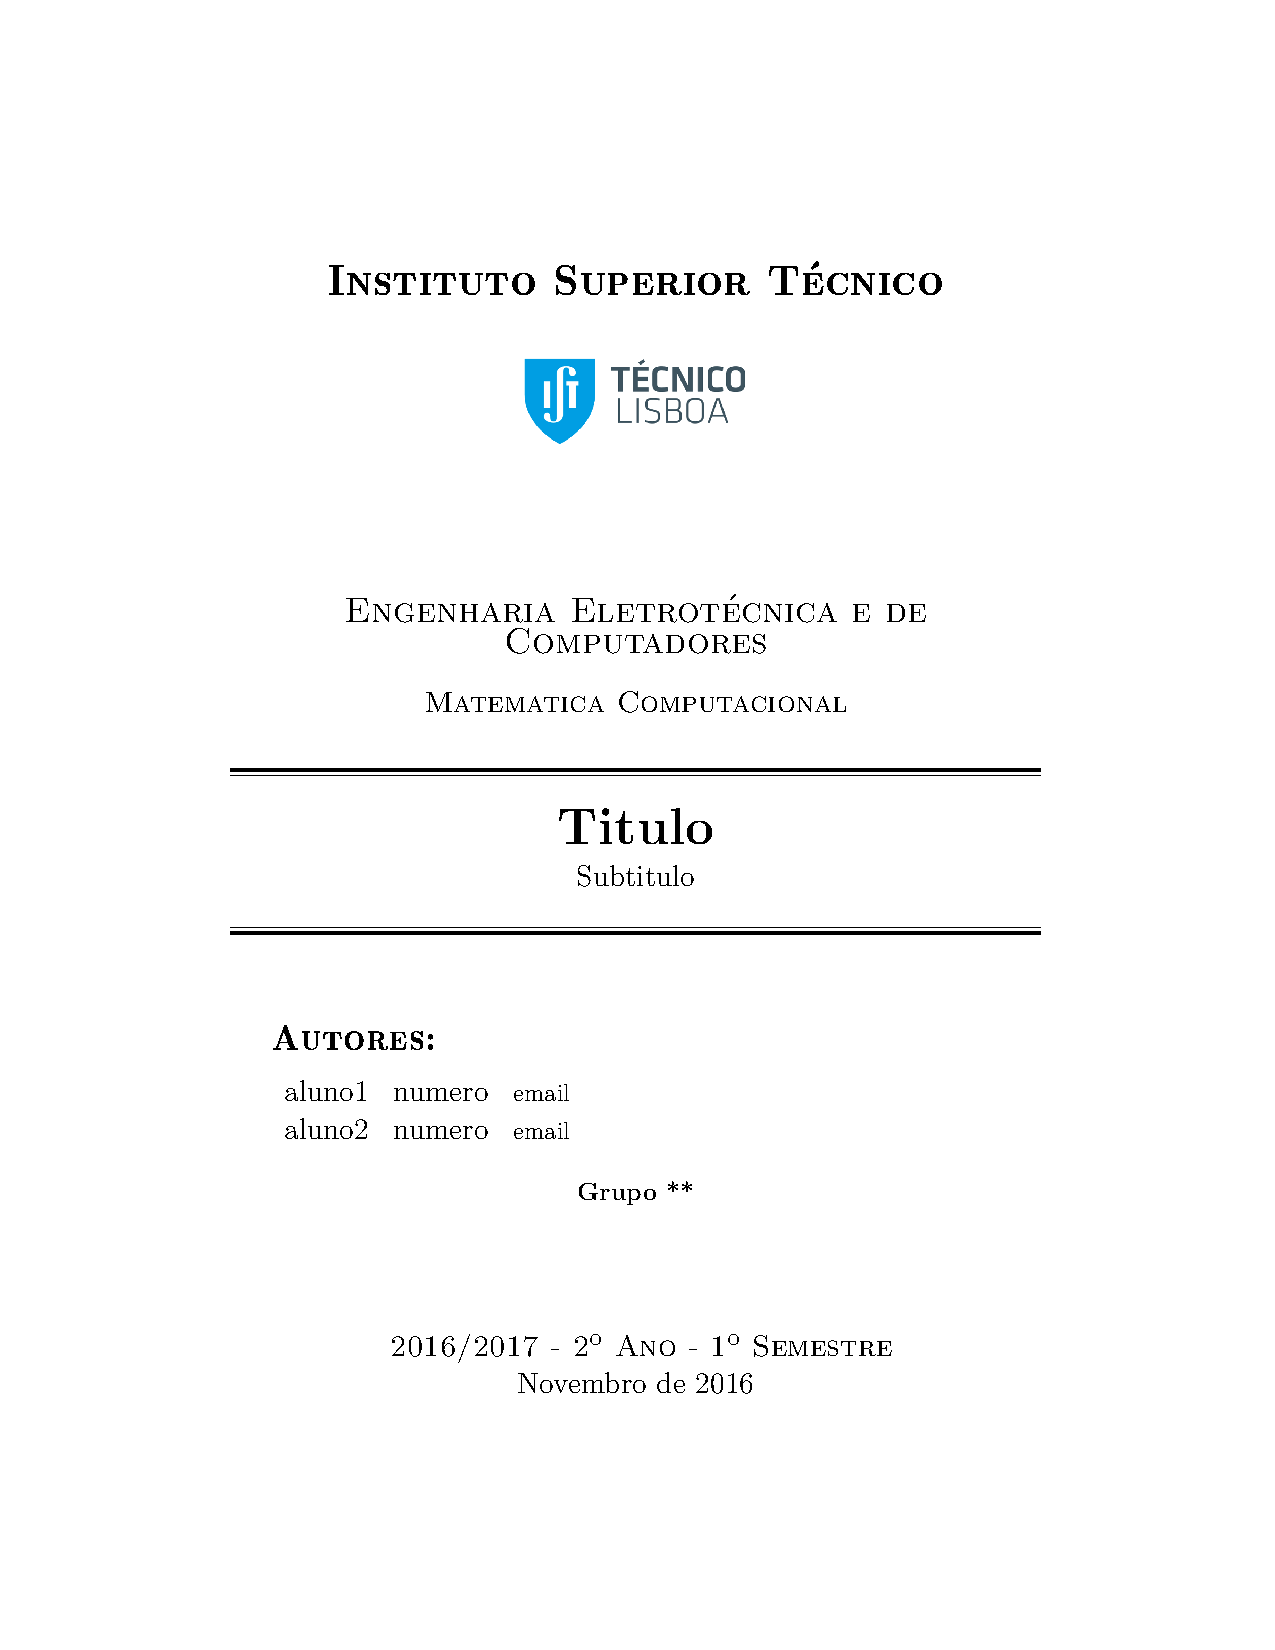
\includepdf[pages={1}]{capa/capa.pdf}

\section{Pergunta 1}
	\begin{equation} \label{init}
		h(\lambda) = \lambda + 15.5 - 2\cosh(\lambda\tau)
	\end{equation}

	\begin{equation}
		h'(\lambda) = 1 - 2\sinh(\tau\lambda) = 1 - \tau(e^{\tau\lambda} - e^{-\tau\lambda})
	\end{equation}

	\begin{equation}
		h''(\lambda) = -2\tau^2\cosh(\tau\lambda) = -\tau^2(e^{\tau\lambda} + e^{-\tau\lambda})
	\end{equation}

	\par
	Analisemos o sinal de $h''(\lambda)$:
	$$\tau > 0$$
	\begin{equation} \label{eq:1_2nd_der_sign}
	\begin{split}
		e^{\tau\lambda} + e^{-\tau\lambda} > 0 &\implies h''(\lambda) < 0, \forall \lambda
	\end{split}
	\end{equation}

	\par
	Pelo Teorema de Rolle e pela inequação \eqref{eq:1_2nd_der_sign} podemos afirmar que
	$h(\lambda)$ tem no máximo duas raízes. Provemos que $h(\lambda)$ tem no mínimo duas raízes sem perda de generalidade.

	\begin{equation}
		h(0) = 0 + 15.5 - 2\cosh(0\tau) = 13.5 > 0
	\end{equation}

	\begin{equation}
	\begin{split}
		\lim_{x \to +\infty} h(\lambda)
		&= \lim_{x \to +\infty} (\lambda + 15.5 - 2\cosh(\lambda)) \\
		&= \lim_{x \to +\infty} e^{\tau\lambda} \bigg(\frac{\lambda}{e^{\tau\lambda}} + \frac{15.5}{e^{\tau\lambda}} - \frac{2\cosh(\lambda)}{e^{\tau\lambda}}\bigg) \\
		&= e^{+\infty} (0 + 0 - 1) = -\infty < 0
	\end{split}
	\end{equation}

	\par
	Analogamente para  $-\infty$ :

	\begin{equation}
	\begin{split}
		\lim_{x \to -\infty} h(\lambda)
		&= \lim_{x \to -\infty} (\lambda + 15.5 - 2\cosh(\lambda)) \\
		&= \lim_{x \to -\infty} e^{-\tau\lambda} \bigg(\frac{\lambda}{e^{-\tau\lambda}} + \frac{15.5}{e^{-\tau\lambda}} - \frac{2\cosh(\lambda)}{e^{-\tau\lambda}}\bigg) \\
		&= e^{+\infty} (0 + 0 - 1) = -\infty < 0
	\end{split}
	\end{equation}

	\par
	Assim, como $h(\lambda)$ é contínua, pelo teorema de Bolzano conclui-se que $h(\lambda)$ tem no mínimo duas raízes, uma positiva e uma negativa. Logo, como $h(\lambda)$ tem no máximo duas raízes, tem exatamente duas raízes.
	\par
	Se $\tau = 0$:
	\begin{equation}
	\begin{split}
		h(\lambda) &= \lambda + 13.5 = 0 \Leftrightarrow \\
		\Leftrightarrow h &= -13.5
	\end{split}
	\end{equation}
	\par
	Por outro lado, se $\tau$ for muito grande, existirá sempre um $\lambda$ arbritariamente perto de $0^-$ tal que:
	\begin{equation}
	\begin{split}
		\lambda + 15.5 &= 2cosh(\lambda\tau) \Leftrightarrow \\
		\Leftrightarrow h(\lambda) &= 0, \lambda < 0
	\end{split}
	\end{equation}
	\par
	Assim, a raiz negativa estará contida no intervalo $]-13.5, 0[, \forall \tau > 0$.


\section{Pergunta 2}
\subsection*{a)}
	\begin{equation} \label{2a}
	\begin{split}
		g(\lambda) &= \lambda - 0.1(\lambda + 15.5 - 2cosh(0.8\lambda)) \Leftrightarrow \\
		\Leftrightarrow g(\lambda) &= 0.9\lambda - 1.55 + 0.2cosh(0.8\lambda)
	\end{split}
	\end{equation}

	\par
	A raiz positiva $z_2$ de \eqref{init} equivale a um ponto fixo de \eqref{2a} e será do tipo repulsor sse:
	$$|g'(z_2)| > 1$$

	\begin{equation}
		g'(\lambda) = 0.9 + 0.16sinh(0.8\lambda)
	\end{equation}

	\begin{equation} \label{2a_2nd_der}
		g''(\lambda) = 0.128cosh(0.8\lambda) > 0, \forall \lambda
	\end{equation}

	\par
	De \eqref{2a_2nd_der} vem que $g'(\lambda)$ é estritamente crescente.
	\begin{equation} \label{2a_cres}
	\begin{split}
		g'(0) &> 0 \\
		g(0) &< 0
	\end{split}
	\end{equation}

	% TODO
	TODO: what if g'(z2) = 1 ???
	\par
	De \eqref{2a_cres} vem que $g(\lambda)$ apenas pode intersetar a reta $y = x$ se $g'(\lambda) \geqslant 1$ para $\lambda > 0$.


\subsection*{b)}
\subsection*{c)}
	Programa em anexo.
\subsection*{d)}

\begin{table}[H] \label{pto_fixo}
\setlength{\tabcolsep}{0.5cm} %padding das colunas
\renewcommand{\arraystretch}{1.5} %padding das linhas
\centering
\caption{Metodo do ponto fixo}
\label{my-label}
\begin{tabular}{|c|c|c|}
 $n$ & $\lambda _n$ &  $| \lambda _{n+1} - \lambda _n |$ \\\hline
 0& -3.000000000000000 & -  \\
 1& -3.138610566606898 & 0.138610566606898 \\
 2& -3.135043175725743 & 0.003567390881155 \\
 3& -3.135319148437489 & 0.000275972711746 \\
 4& -3.135298158933368 & 0.000020989504121 \\
 5& -3.135299757437974 & 0.000001598504606 \\
 6& -3.135299635712395 & 0.000000121725579 \\
\end{tabular}
\end{table}

\subsection*{e)}
\subsubsection*{i.)}

\begin{table}[H] \label{convergencia}
\setlength{\tabcolsep}{0.5cm} %padding das colunas
\renewcommand{\arraystretch}{1.5} %padding das linhas
\centering
\caption{Convergencia}
\label{my-label}
\begin{tabular}{c|c|c|c}

TODO: porque e que os valors em 0 e em 1 são iguais
 $n$ & $\frac{|e_{n+1}|}{|e_n|^{1/2}}$ &  $\frac{|e_{n+1}|}{|e_n|}$ & $\frac{|e_{n+1}|}{|e_n|^{2}}$ \\\hline
 0& 0.009001228832727  & 0.024471099844949 & 0.000180865969935 \\
 1& 0.009001228832727  & 0.024471099844949 & 0.000180865969935 \\
 2& 0.004457019736082  & 0.077458574287344 & 0.023394802475624 \\
 3& 0.001218451139231  & 0.076084871362003 & 0.296673459104577 \\
 4& 0.000334315531198  & 0.075682869509848 & 3.878641714344468 \\
 5&  &  & \\
 6&  &  & \\
\end{tabular}
\end{table}


\subsubsection*{ii.)}
\subsection*{f)}

\section{Pergunta 3}

\section{Pergunta 4}

\section{Anexo}

\end{document}
